\documentclass[]{article}
\usepackage{caption}
\usepackage{graphicx}
\graphicspath{ {./images/} }
\usepackage{fancyhdr}
%opening
\title{Preparing Moth Specimens for Dissection}
\author{Dr. Paul J. Palmer}



\pagestyle{fancy}
\makeatletter
\let\runauthor\@author
\let\runtitle\@title
\makeatother
\chead{\runtitle}
\lfoot{\runauthor}
\rfoot{\today}





\begin{document}

%\maketitle
\pagenumbering{gobble}
%\begin{abstract}
%
%\end{abstract}

%\section*{Pitfall traps for spider recording}

%\begin{center}
%	\centering
%	\includegraphics[width=0.3\linewidth]{images/pitfall}\hfill
%	\includegraphics[width=.3\textwidth]{images/alcohol}\hfill
%	\includegraphics[width=.3\textwidth]{images/complete}\hfill
%	\captionof{figure}{Placing the pitfall trap: Place the pitfall cup in a carefully dug hole; Fill the collector cup with 30 mL of food grade  \textit{Mono~Propylene~Glycol} and  place the inside the pitfall; Cover with the rain shield leaving a vertical gap of about 10~mm. }
%	
%\end{center}

These instructions explain how to prepare moth specimens for confirmation of  identification (ID) by microscopic examination. These are my own preferences, but other workers will probably accept specimens prepared in this way. ID often requires examination of both external and internal features so the whole specimen should be preserved in a near perfect condition as possible. Dissection of the genitalia requires removal of the abdomen and separation of the reproductive organs and their arrangement on a microscope slide. This is only possible if the specimen is completely dessicated since the presence of any moisture will result in decay and the growth of moulds obscuring the features required for ID. Traditionally specimens were presented set on pins in a perfectly dehydrated state ready for examination. Specimen details were included  on labels mounted on the same pin. Postal boxes specifically for  sending pinned specimens through the mail are still available from specialist suppliers.

Unmounted specimens should be stored in suitable tubes treated in the following way:
\begin{description}
	\item[Label] A label should be placed \textbf{inside the tube} recording: Who, What, Where, When and How. Figure~\ref{InternalLabel} illustrates how labels are used and why they must be inside the specimen tube.
	\item[Freezer] A minimum of 48 hours in a domestic freezer will ensure that the specimen is dead along with any mites that may be present. There is no harm in exceeding this time.
	\item[Dehydration] Exposure to dry air is needed to remove all moisture. The tubes should be uncovered and stoppered with cotton wool and left for several weeks or longer. If the dessication is carried out in the freezer, then the tubes should be brought up to room temperature and left for several hours before the lids are put in place.
	\item[Post] The tubes may be posted to: Paul Palmer, 136 Burton Road, Melton Mowbray, Leicestershire LE13 1DL. An advance note is appreciated \\ (\texttt{palmerpjp@gmail.com}) and by arrangement, callers are always welcome.
\end{description}


% TODO: \usepackage{graphicx} required
\begin{center}
	\centering
	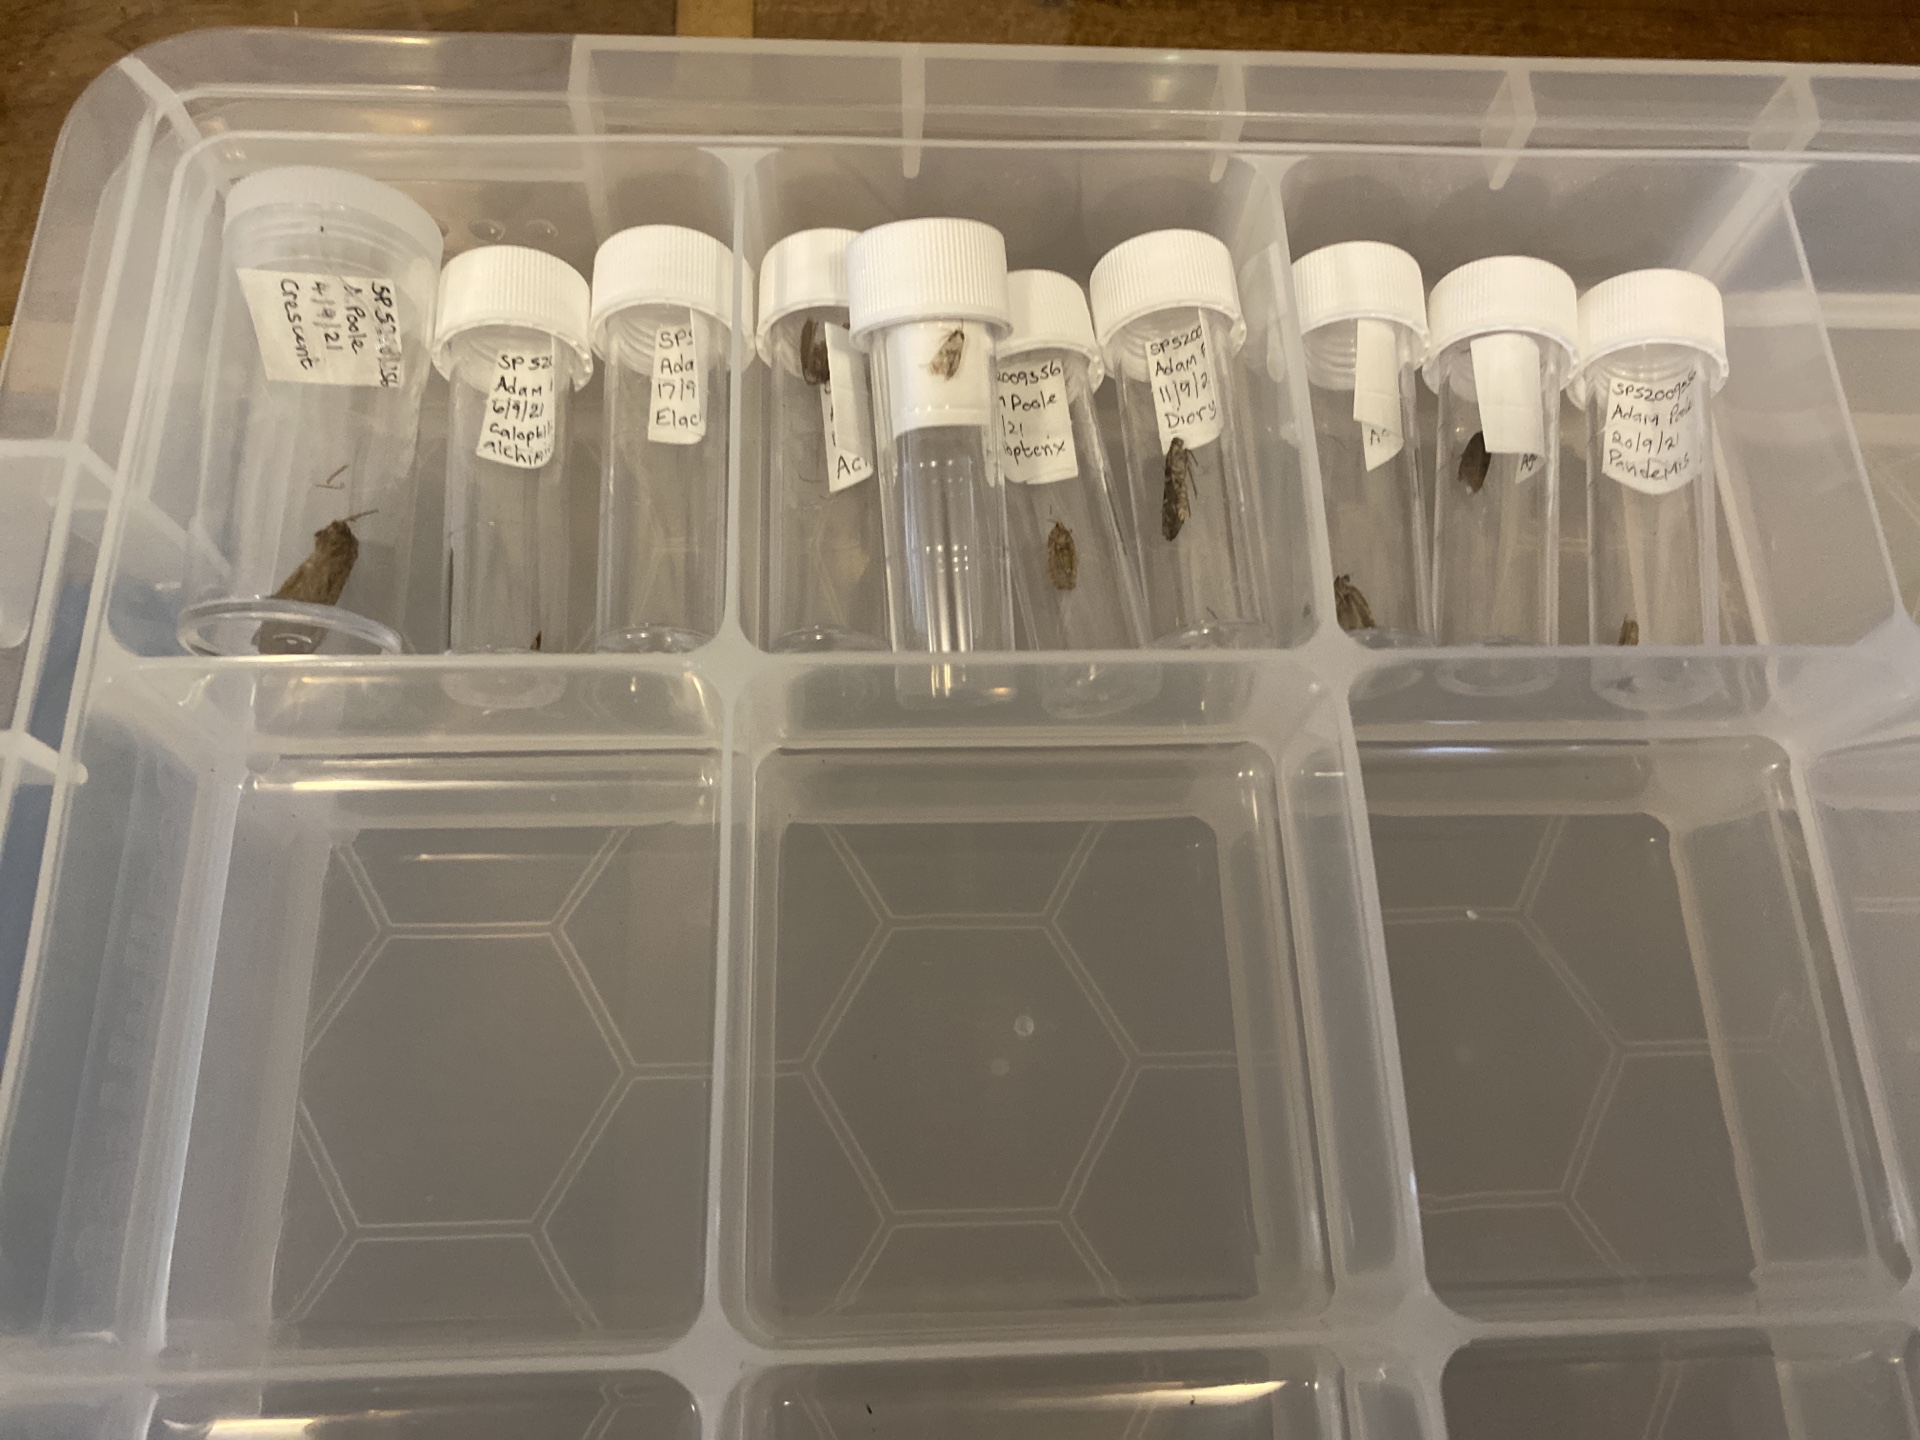
\includegraphics[width=0.3\linewidth]{images/specimens}\hfill
	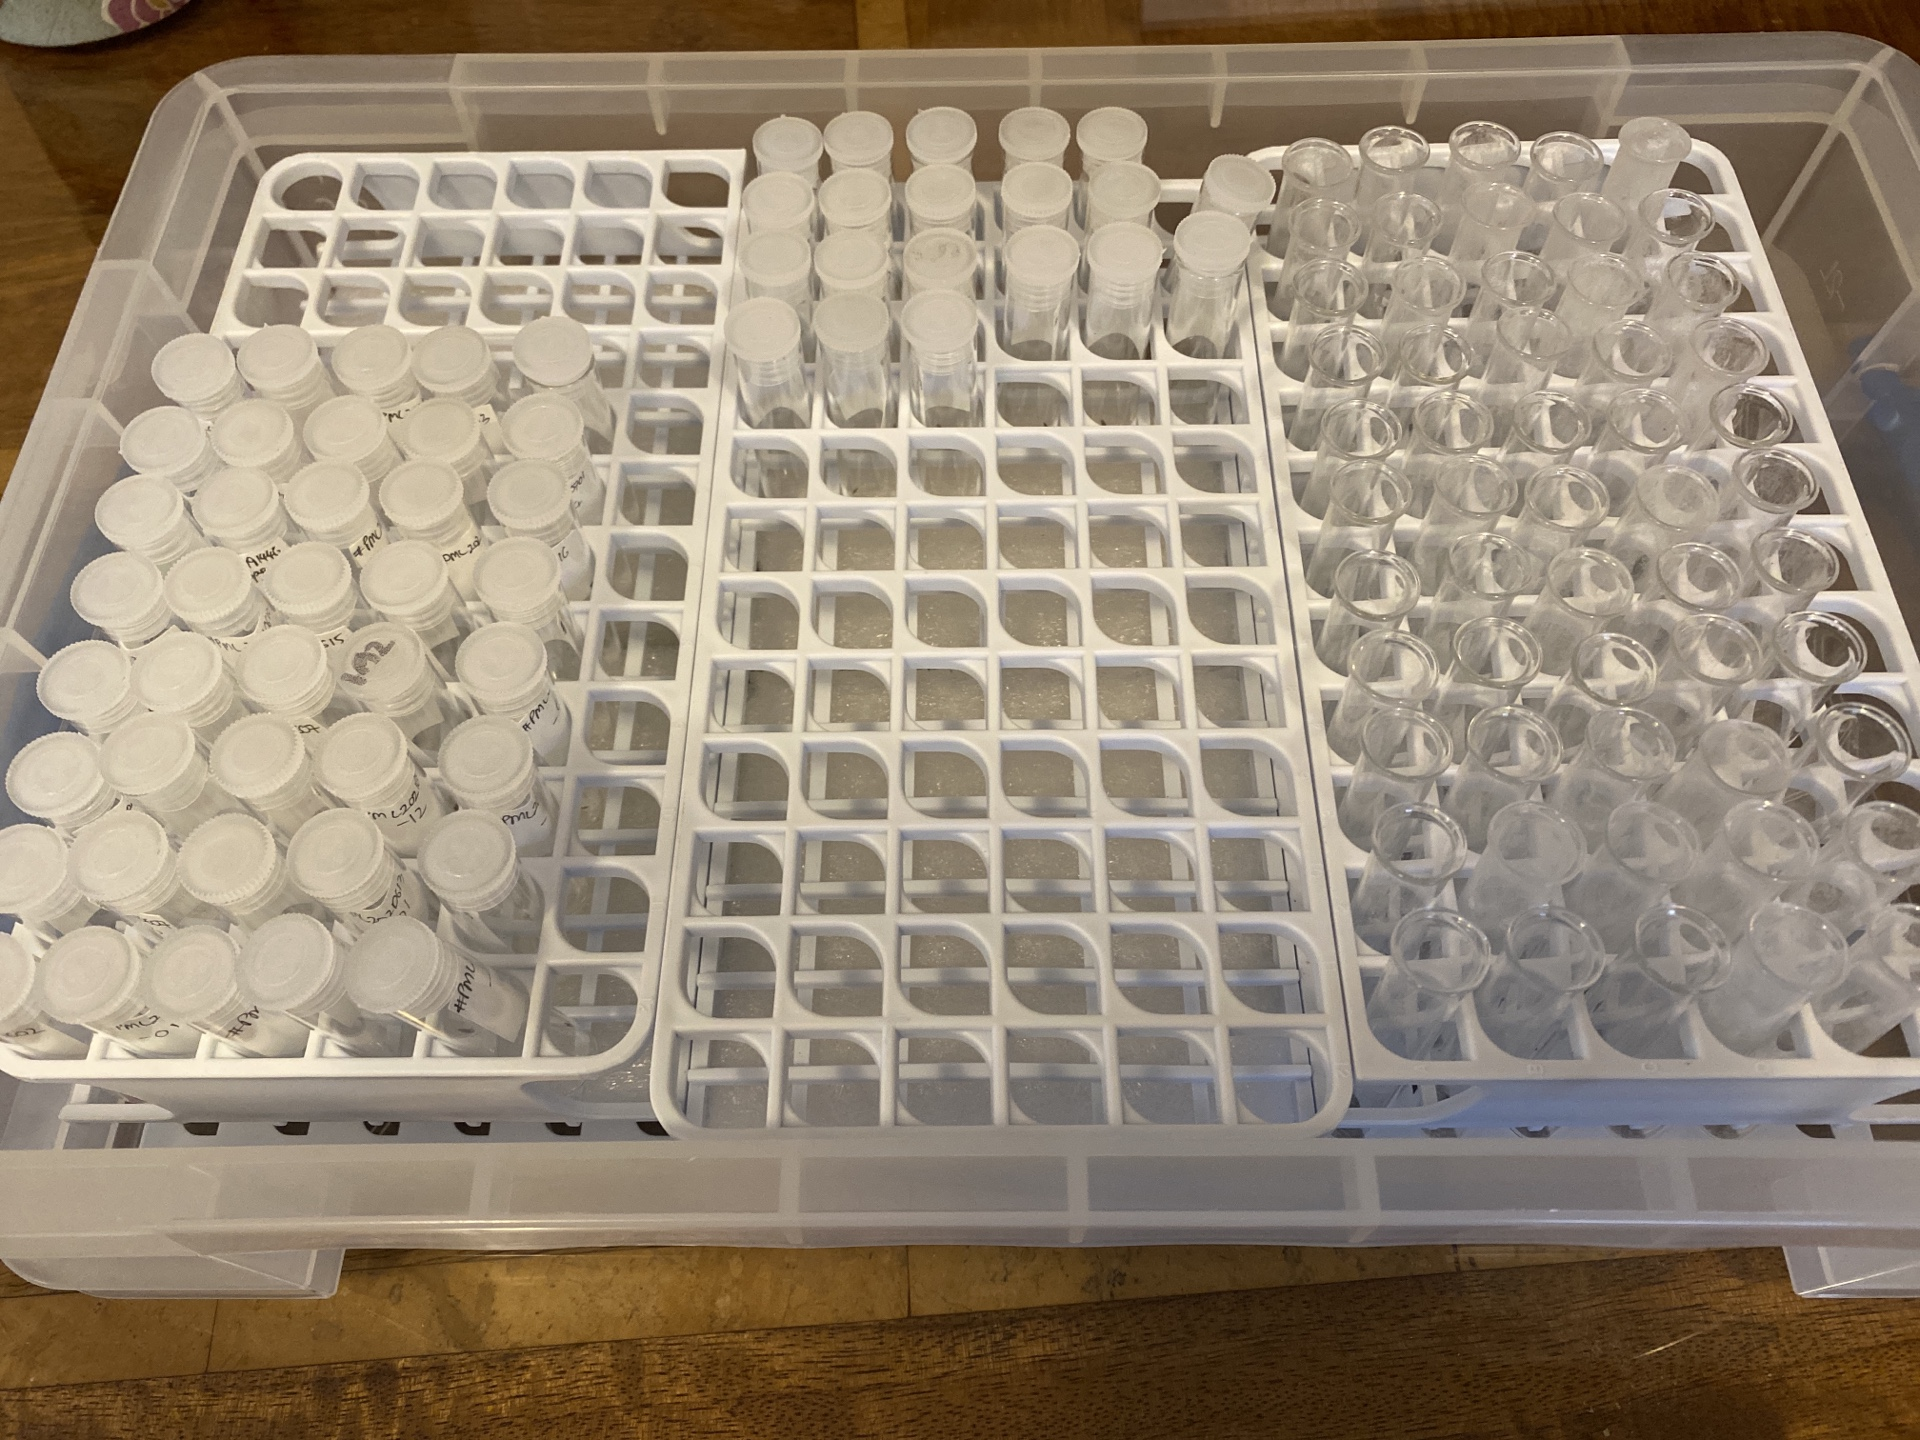
\includegraphics[width=.3\textwidth]{images/prepared}\hfill
	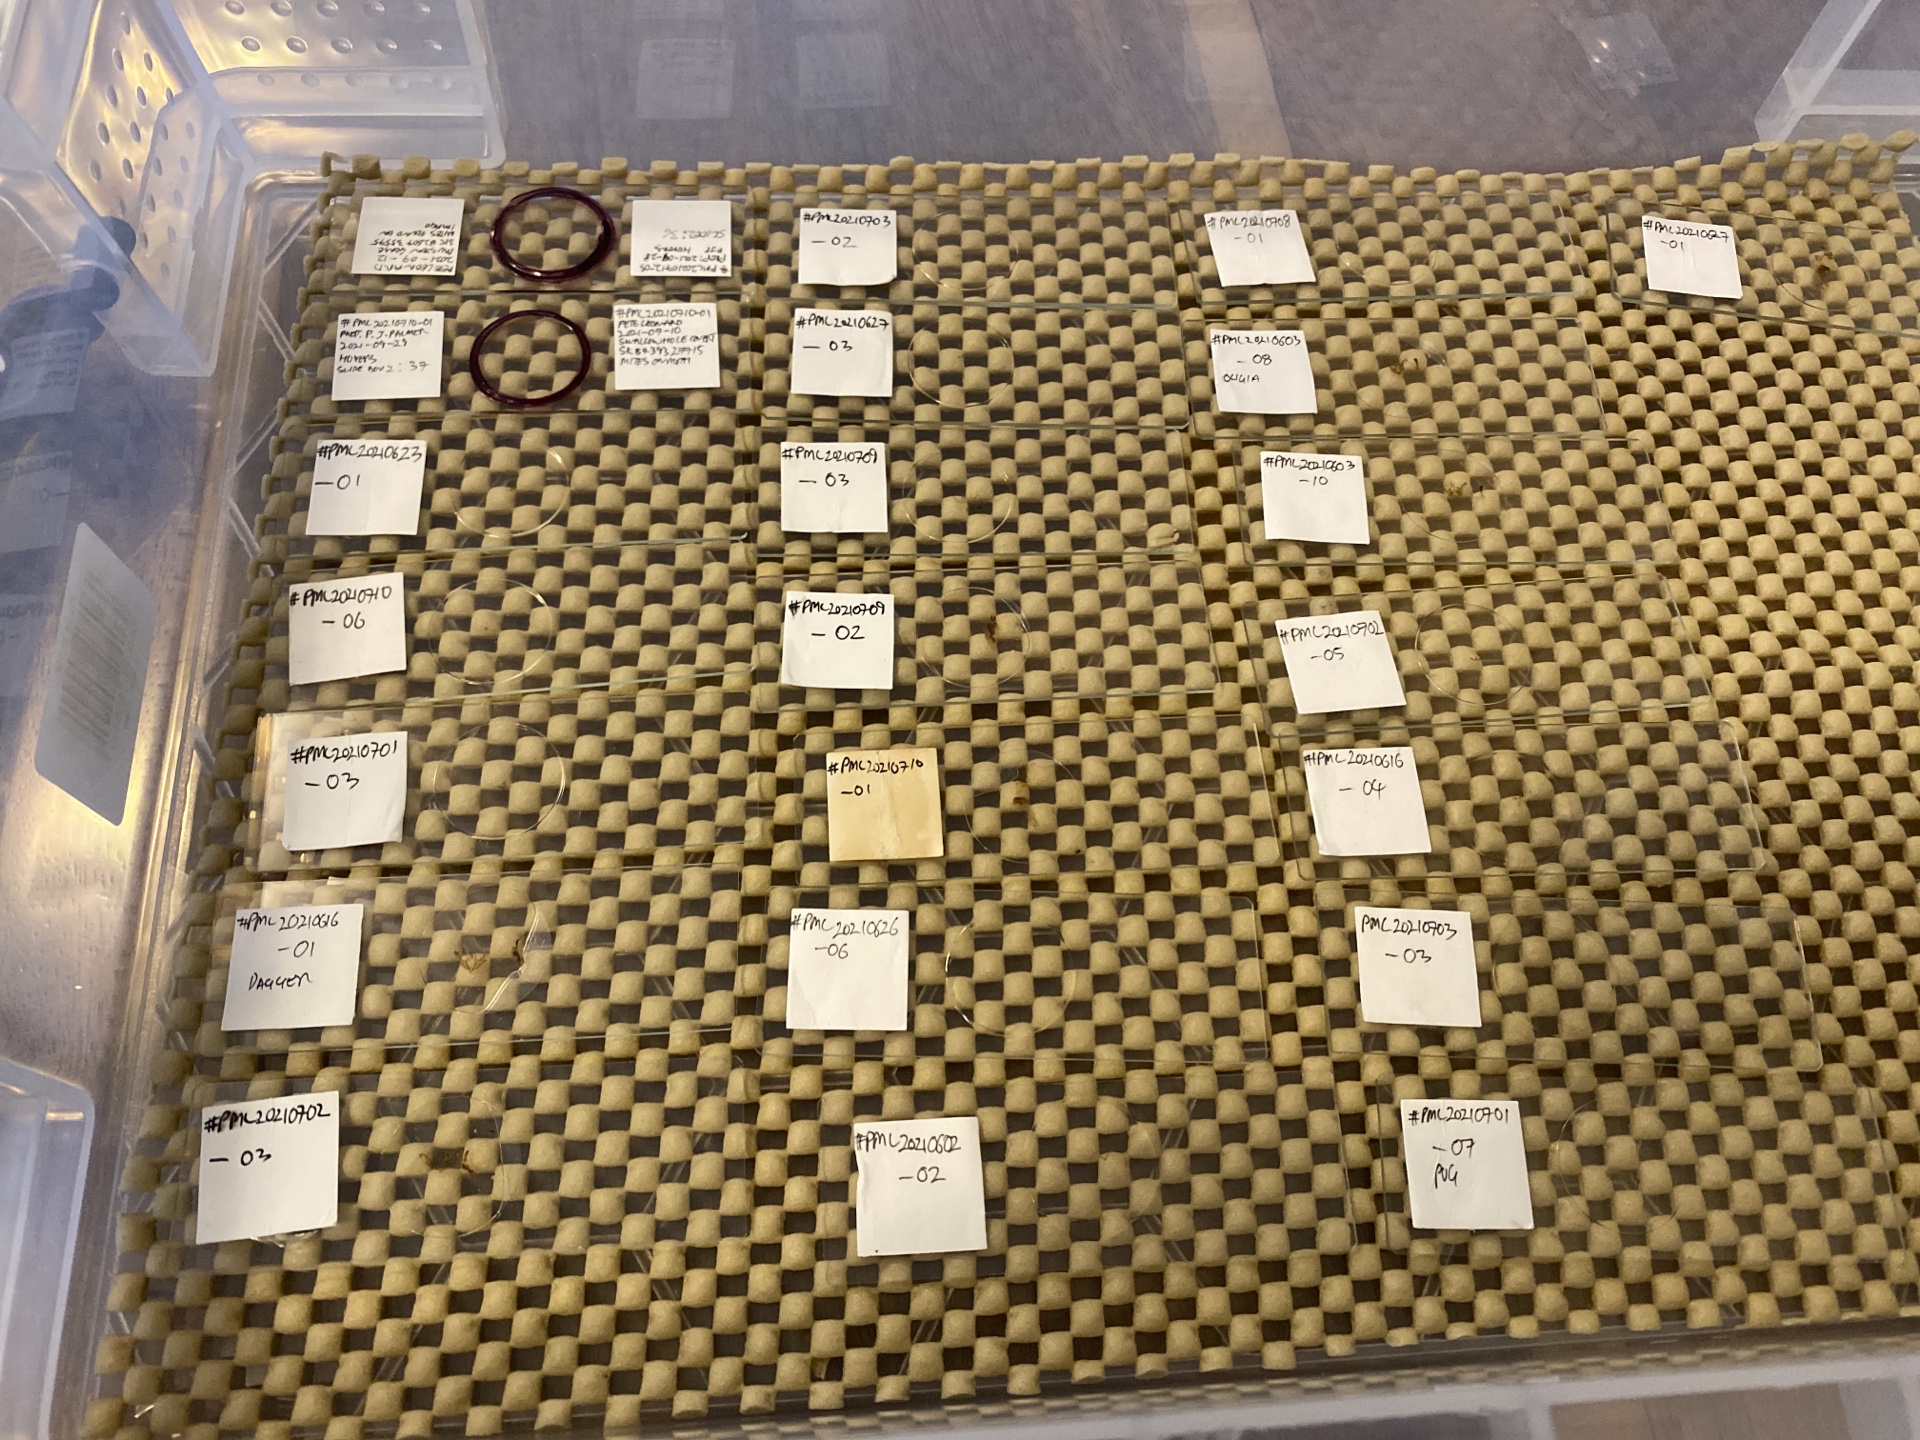
\includegraphics[width=.3\textwidth]{images/slides}\hfill
	\captionof{figure}{From left to right: Specimens as recieved for examination; Once photographed and catalogued each specimen is placed in a standard tube along with its label; After dissection, the label is glued to the microscope slide.}
	\label{InternalLabel}
\end{center}




\end{document}
